\section{Implementazione}\label{sec:implementazione}

In questa sezione verranno trattati gli aspetti inerenti all'implementazione hardware e software legata allo sviluppo del sistema:
in primo luogo saranno velocemente presentate le tecnologie utilizzate all'interno di una o più delle entità in gioco nel sistema,
successivamente verrà dedicata una \nameCref{subsec:cloud} a ciascuna di queste dove saranno analizzate nello specifico l'architettura e le funzionalità di dettaglio.

La configurazione di rete finale è riportata in \Cref{fig:network}.

\begin{figure}[H]
  \centering
  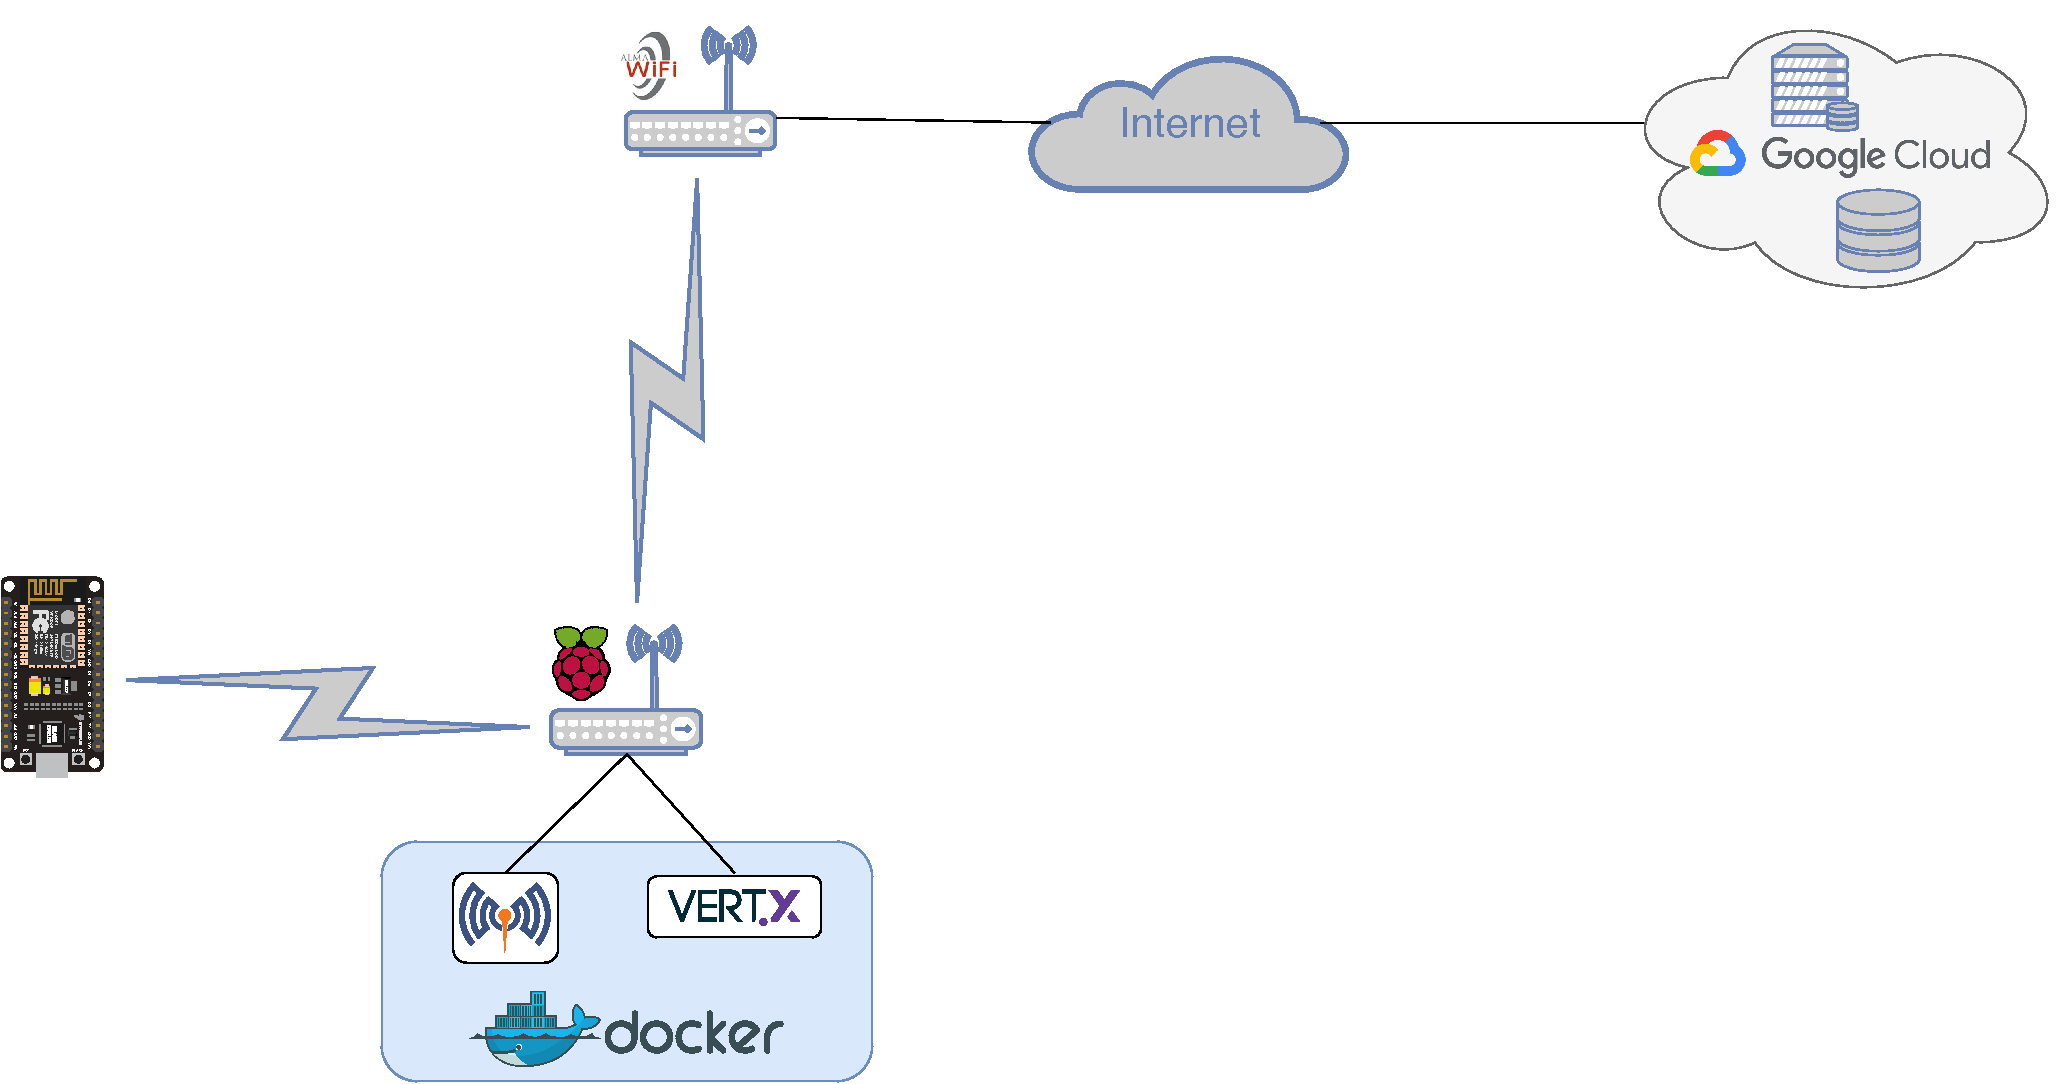
\includegraphics[width=\textwidth]{res/out/network.pdf}
  \caption{Rappresentazione della configurazione di rete finale realizzata}%
  \label{fig:network}
\end{figure}

\subsection{Tecnologie Utilizzate}

Di seguito sono riportate in un elenco le tecnologie più rilevanti utilizzate per l'implementazione del progetto.

\begin{description}
  \item[Typescript \& Angular]
    Per la realizzazione dei frontend web del server cloud e del server edge, è stato impiegato il framework Angular con il linguaggio consigliato Typescript.
    \strong{Typescript}\footnote{\url{https://www.typescriptlang.org/}} è un Super-set di JavaScript ES6 e, come tale, è un linguaggio di scripting orientato agli oggetti e agli eventi;
    \strong{Angular}\footnote{\url{https://angular.io/}}, invece, è un framework open source per lo sviluppo di applicazioni web con licenza MIT, realizzato in Typescript e sviluppato principalmente da Google.
    Tramite Angular è stato possibile realizzare SPA autonome reattive e leggere.
  \item[Mosquitto\footnotemark]\footnotetext{\url{https://mosquitto.org/}}
    Come broker MQTT è stato scelto \strong{Eclipse Mosquitto}, soluzione leggera e open-source compatibile con le più recenti versioni del protocollo.
  \item[Cloud Firestore]
    Per memorizzare i dati raccolti è stato utilizzato \strong{Cloud Firestore}, un database flessibile e scalabile per lo sviluppo di dispositivi mobili, Web e server da Firebase e Google Cloud Platform.
  \item[Kotlin\footnotemark]\footnotetext{\url{https://kotlinlang.org/}}
    Per l'implementazione del server di backend e la gestione delle API è stato utilizzato \strong{Kotlin}, un linguaggio di programmazione general purpose, multi-paradigma (object-oriented e funzionale), open source sviluppato dall'azienda di software JetBrains e basato su JVM\@.
  \item[Vertx\footnotemark]\footnotetext{\url{https://vertx.io/}}
    Libreria utilizzata all’interno dei componenti che si basano su una JVM, mette a disposizione una serie di primitive e strutture che non solo consentono di modellare un'architettura asincrona e basata sullo scambio di messaggi all'interno del singolo componente, ma permette una gestione semplice, veloce e immediata delle chiamate REST e dei messaggi su MQTT\@.

    Tra gli altri si è optato per Vert.x, oltre che per la sua struttura basata sugli eventi asincroni all’interno di un event-loop, per la sua semplicità di deploy.
    A differenza di altri web server più conosciuti all’interno del mondo JVM come Java EE o Spring, Vert.x è totalmente indipendente e non necessita di un servlet container, permettendo perciò un deploy ancora più immediato.
  \item[Docker]
    Per il deploy, sia su Google App Engine che su Raspberry Pi, è stato utilizzato Docker tramite la realizzazione di container dedicati nei quali eseguire il software.
    Anche il deploy di Mosquitto avviene tramite Docker.
\end{description}

\subsection{Backend Cloud}\label{subsec:cloud}

Il backend in Cloud si occupa principalmente di interagire con il database, oltre a fornire le API per l'accesso alle informazioni raccolte in tutte le differenti zone.

La logica implementativa è molto semplice e vede un singolo \text{Verticle} (motore di esecuzione molto simile al pattern ad attori) che si occupa di esporre le API REST e di gestire le interazioni con il database.

Come già specificato in precedenza, il deploy è effettuato su Google App Engine tramite container Docker;
la procedura è documentata in \Cref{app:gcp}.

\subsubsection{OpenAPI}\label{subsub:openapi}

Le API sono documentate tramite standard Swagger/OpenAPI 3.0~\cite{OpenAPIInitiative2018}, il cui documento può essere trovato in \Cref{app:openapi:cloud};
tale documentazione è letta da Vert.x, il quale associa ad ogni \emph{route} un \emph{handler} asincrono specifico.

Per semplicità, le API mettono a disposizione solo le operazioni di aggiunta (tramite metodo \texttt{PUT}) e visualizzazione (tramite metodo \texttt{GET}) di nuove misurazioni, e sono le seguenti:

\begin{itemize}
  \item
    \texttt{/api/devices/\{location\}} modella la risorsa relativa ai dispositivi opportunamente anonimizzati memorizzati nel DB\@.
    Gli oggetti JSON scambiati contengono:
    \begin{itemize}
      \item un campo \texttt{hash-mac} contenente il risultato di una funzione hash eseguita sull'indirizzo MAC individuato;
      \item un campo \texttt{vendor} contentente il nome del produttore risolto a partire dall'indirizzo MAC prima dell'anonimizzazione;
    \end{itemize}
    È possibile specificare una location nel path per filtrare i risultati di un solo edificio; per eseguire le \texttt{PUT} essa è obbligatoria.
  \item
    \texttt{/api/crowd/\{location\}} modella la risorsa relativa alle misurazioni di affollamento memorizzate nel DB\@.
    Gli oggetti JSON scambiati contengono:
    \begin{itemize}
      \item un campo \texttt{time} contenente il timestamp di quanto è stata effettuata la misurazione;
      \item un campo \texttt{zone} contentente la location della misurazione;
      \item un campo \texttt{crowd} contentente il numero di dispositivi rilevati;
    \end{itemize}
    È possibile specificare una location nel path per filtrare i risultati di un solo edificio; per eseguire le \texttt{PUT} essa è obbligatoria.
\end{itemize}

Oltre a queste, sono disponibili altre due API\@:

\begin{itemize}
  \item \texttt{GET} \texttt{/api/vendors} che permette di risolvere i soli vendor;
  \item
    \texttt{POST} \texttt{/api/auth} che permette di ottenere un token JWT che autorizza l'accesso al sistema in scrittura:
    è infatti necessario inviarlo come \emph{bearer authorization header} per poter effettuare le \texttt{PUT} specificate sopra.
\end{itemize}

\subsubsection{Cloud Firestore}

La comunicazione tra il \texttt{Verticle} e il database è gestita tramite un libreria wrapper realizzata per Vert.x.
Essa si interfaccia tramite SDK nativo e fornisce osservabili reattivi con cui interagire in modo asincrono.

Per quanto riguarda la modellazione dei dati all'interno del DB, le collezioni sono definite in modo molto simile alle risorse REST\@.
Sono state realizzate le seguenti collezioni, con i documenti aventi la medesima struttura degli oggetti JSON documentati sopra:

\begin{itemize}
  \item \texttt{crowds} contenente tutte le misurazioni suddivise per zona;
  \item \texttt{devices} contentente tutti i dispositivi rilevati;
  \item \texttt{located-devices} ospitante le informazioni relative ai dispositivi presenti in una certa zona.
\end{itemize}

\subsection{Server Fog}

Il server Fog è stato realizzato con un Raspberry Pi 3 Model B equipaggiato con un ricevitore USB WiFi N.
Il sistema operativo installato è Raspbian Buster; su di esso è stato installato Docker (per l'esecuzione del broker MQTT Mosquitto e del codice di backend) e RaspAP (per poter generare un hotspot locale mantenendo la connessione a internet tramite una seconda rete WiFi).
La procedura di configurazione è documentata in \Cref{app:raspi}.

\subsubsection{Backend Fog}

Il backend realizzato con Vert.x e Kotlin per definire il comportamento del server Fog è costituito da due \texttt{Verticle} principali:

\begin{itemize}
  \item
    \texttt{BackendVerticle}, che ha un comportamento molto simile all'omonima classe descritta alla \Cref{subsec:cloud}.
    La principale differenza sta nel fatto che anziché comunicare direttamente col DB, essa comunica con il cloud, risolvendo le informazioni da remoto.
  \item
    \texttt{MqttVerticle}, che effettua la sottoscrizione al broker MQTT su cui i sensori IoT pubblicano le informazioni, occupandosi di gestire l'anonimizzazione dei MAC e la loro pubblicazione tramite chiamate API\@.
    Come era stato pianificato nella fase di \labelcref{sec:project} alla \Cref{sec:project} (\Cref{fig:measure}), alla pubblicazione su MQTT esso effettua una chiamata HTTP che viene gestita da \texttt{BackendVerticle}.
\end{itemize}

\subsection{Frontend (Cloud \& Fog)}

Lo sviluppo dell'interfaccia web dell'applicativo è stato realizzato attraverso il framework Angular utilizzando il linguaggio Typescript.
Si è proceduto principalmente per step successivi, cercando di realizzare inizialmente uno scheletro iniziale dei vari componenti web, per poi andare a migliorare aggiungendo dettagli e features di volta in volta.

\subsubsection{Frontend Cloud}

L'interfaccia web per la parte Cloud consiste in una rappresentazione dei dati attraverso due grafici, entrambi realizzati grazie alla libreria \texttt{Chart.js}: uno a linee ed uno a torta.
Il grafico a linee rappresenta l'andamento nel tempo (nell'intervallo prestabilito di 2 ore) dell'affollamento rilevato per tutti i potenziali fog (ognuno rappresentato da una linea); sull'asse delle ascisse il tempo, su quello delle ordinate il quantitativo di dispositivi trovati.
Il grafico a torta viene utilizzato per mostrare una statistica relativa ai vari vendor (ricavabili dal MAC address) di ogni dispositivo rilevato.

\begin{figure}[H]
  \centering
  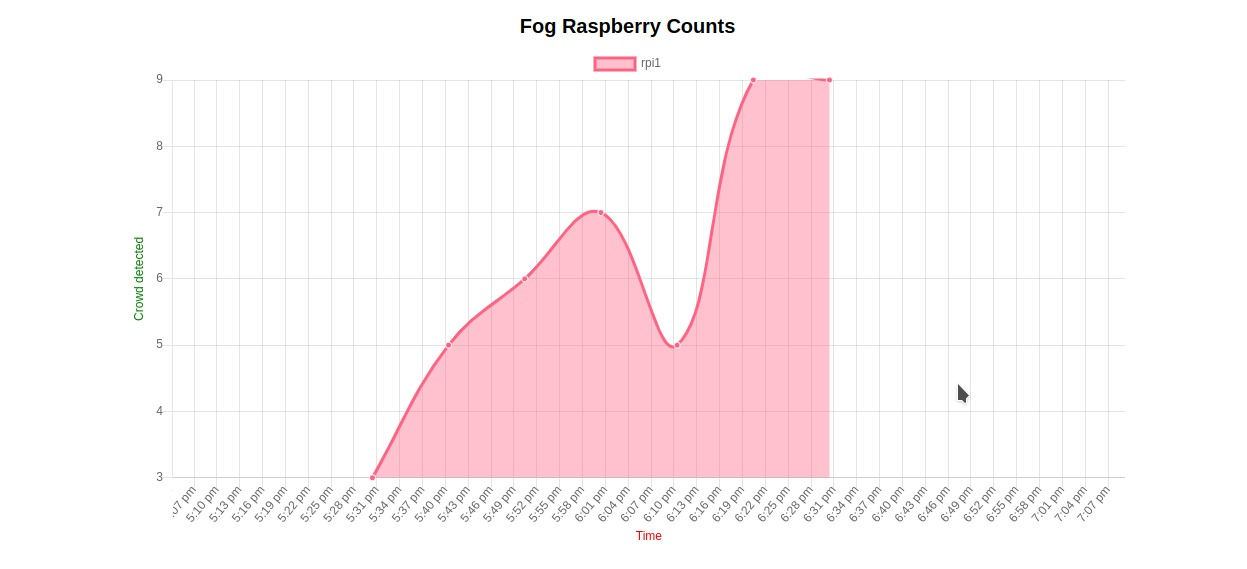
\includegraphics[width=\textwidth]{res/fig/cloud-chart.jpg}
  \caption{Grafico a linee relativo all'affollamento delle diverse zone (qui solo una, \texttt{rpi1})}%
  \label{fig:cloud-chart}
\end{figure}

\begin{figure}[H]
  \centering
  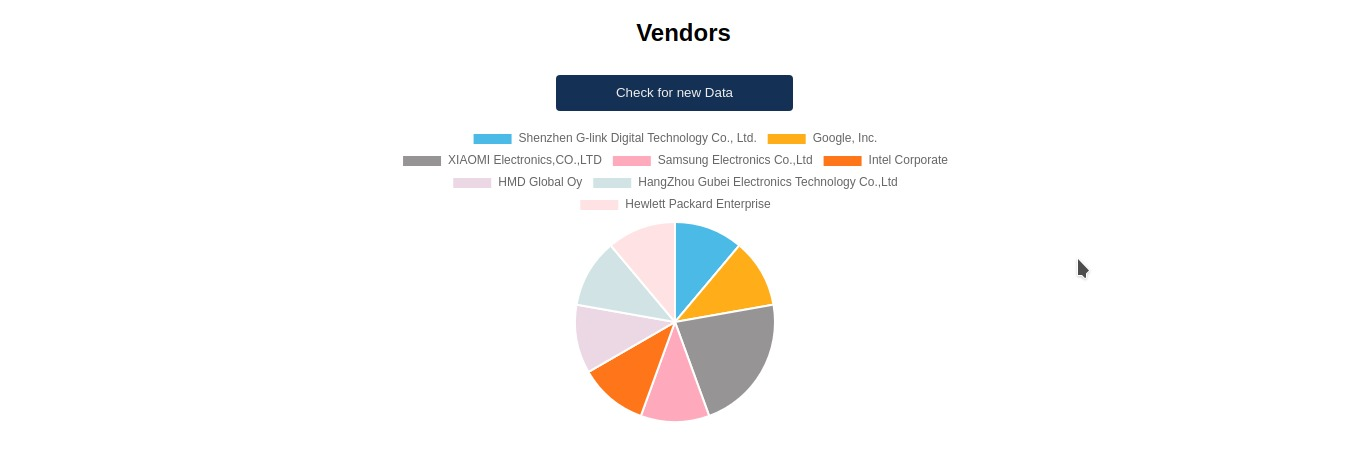
\includegraphics[width=\textwidth]{res/fig/cloud-pie.jpg}
  \caption{Grafico a torta rappresentante il rapporto di frequenza dei differenti vendor}%
  \label{fig:cloud-pie}
\end{figure}

\subsubsection{Frontend Fog}

L'interfaccia web per la parte Fog consiste in una rappresentazione tabellare dei dispositivi rilevati (comprendente vendor e un hash del MAC address per ogni dispositivo), un grafico a linee concettualmente simile a quello sviluppato nel frontend cloud ed un contatore del totale dei dispositivi trovati.

\begin{figure}[H]
  \centering
  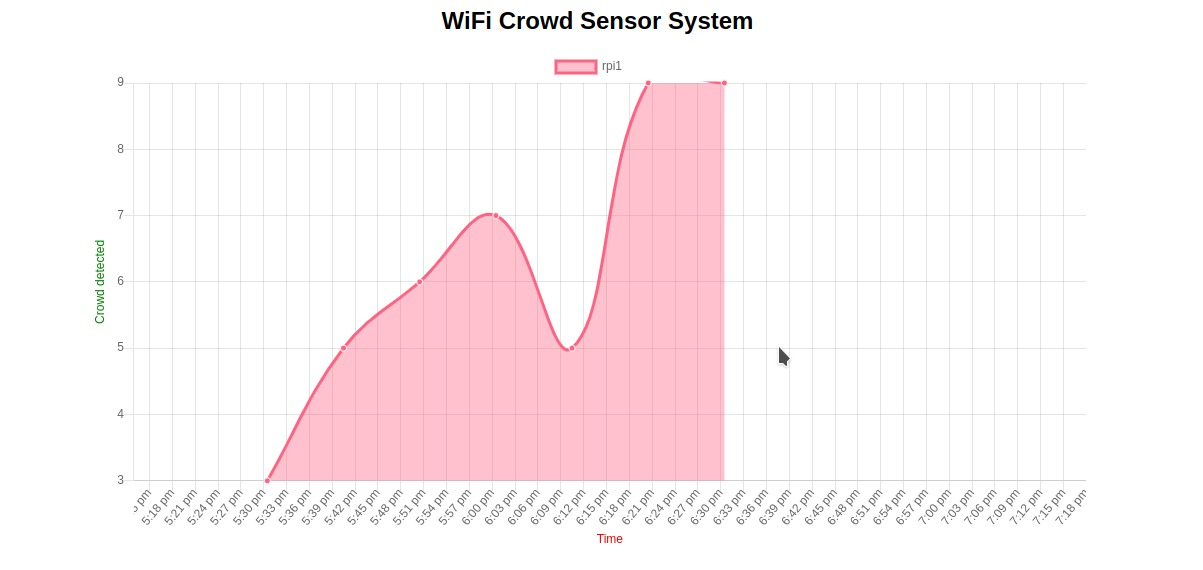
\includegraphics[width=\textwidth]{res/fig/fog-chart.jpg}
  \caption{Grafico a linee relativo all'affollamento della zona locale al Fog server}%
  \label{fig:fog-chart}
\end{figure}

\begin{figure}[H]
  \centering
  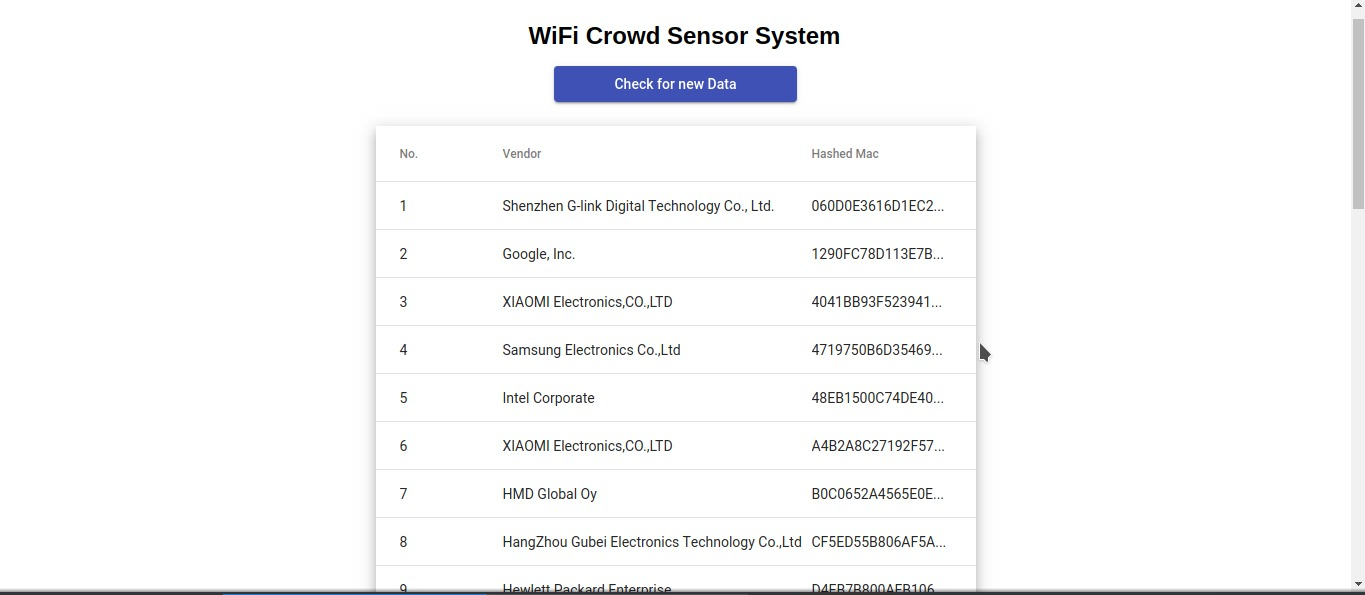
\includegraphics[width=\textwidth]{res/fig/fog-table.jpg}
  \caption{Lista dei differenti vendori rilevati con l'ultima misurazione}%
  \label{fig:fog-table}
\end{figure}

\subsection{Sensori IoT}

La parte di dialogo con l'hardware riguarda soprattutto l'implementazione dei sensori.
Come implementazione fisica si è scelto di utilizzare un modulo Espressif ESP8266, fornito tramite devkit NodeMCU e programmato tramite framework Arduino.
Nel 2016, Ray Brunette su hackster.io\footnote{\url{https://www.hackster.io/rayburne/esp8266-mini-sniff-f6b93a}} ha documentato l'utilizzo di API non pubblicamente descritte che permettevano al dispositivo di funzionare in ``modalità promiscua'',
implementando un semplice scanner di pacchetti ``probe request'' (visibile in \Cref{fig:probe}).

\begin{figure}[H]
  \centering
  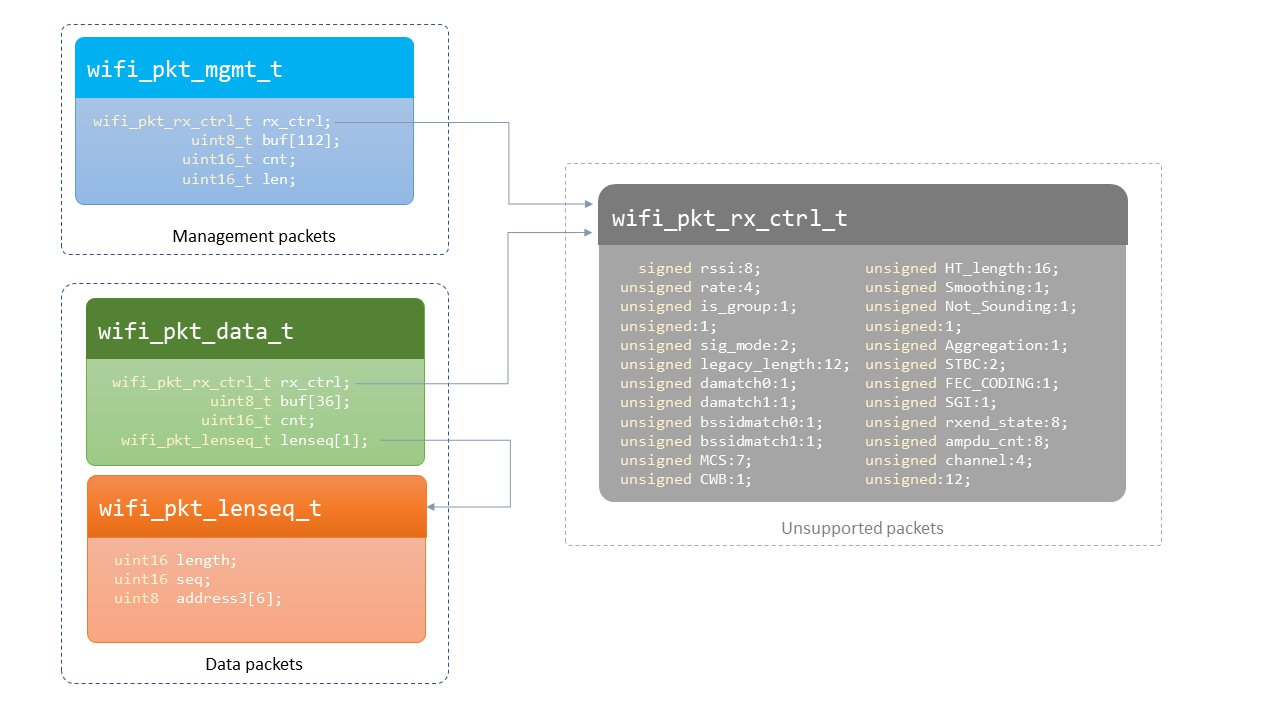
\includegraphics[width=\textwidth]{res/fig/sniffer.jpg}
  \caption{Struttura del pacchetto ``probe request''}%
  \label{fig:probe}
\end{figure}

A partire dal suo codice, pubblicato sotto licenza MIT, sono state realizzate numerose implementazioni differenti;
la nostra è una di quelle.
A partire dal suo codice, è stata aggiunta la comunicazione tramite MQTT e velocizzata la scansione, diminuendo il tempo dedicato a ciascun canale.

Il sensore, ciclicamente, scansiona ogni canale, mantenendo traccia dei dispositivi individuati in ciascuno di esso.
Terminato il ciclo, esso si collega alla rete generata dal Raspberry Pi e pubblica il vettore di indirizzi MAC sul topic \texttt{Sniffer} via MQTT\@.
